%%%%%%%%%%%% MANUAL DE USO %%%%%%%%%%%%

\begin{center}
	{\fboxrule=4pt \fbox{\fboxrule=1pt
		\fbox{\LARGE{\bfseries 1. Forma de Compilación en Code::Blocks}}}} \\
	\addcontentsline{toc}{chapter}{1. Forma de Compilación en Code::Blocks IDE}
	\setcounter{chapter}{1}
	\setcounter{section}{0}
	\rule{15cm}{0pt} \\
\end{center}
\begin{figure}[H]
	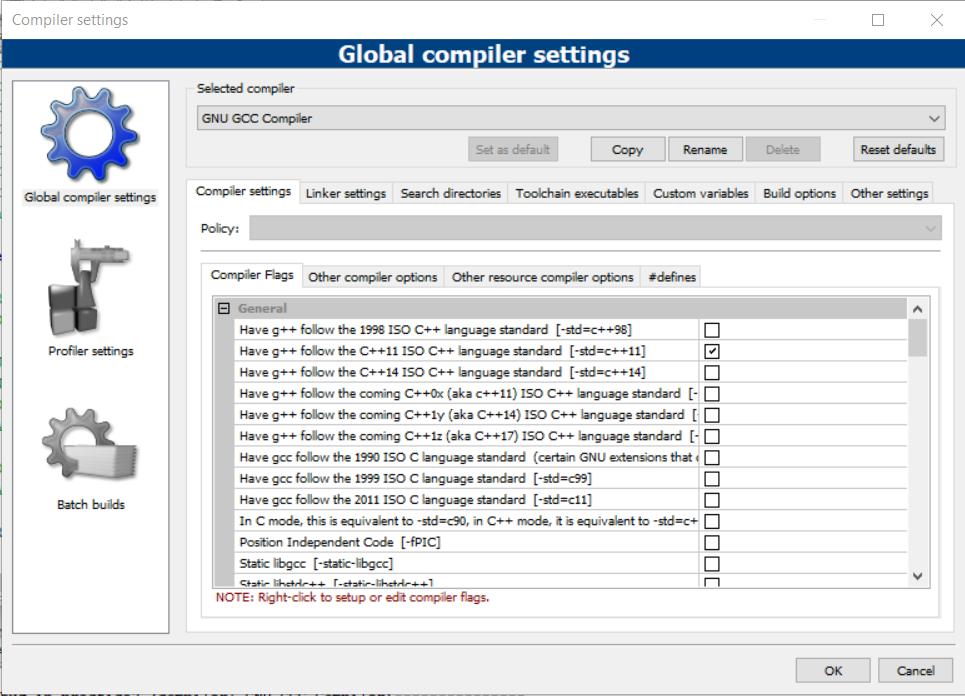
\includegraphics[width=\textwidth]{compilar}
	\centering
	\caption{Figura.}
    \label{fig:SBR}
\end{figure}
\begin{center}
	{\fboxrule=4pt \fbox{\fboxrule=1pt
		\fbox{\LARGE{\bfseries 2. Forma de Ejecución}}}} \\
	\addcontentsline{toc}{chapter}{2. Forma de Ejecución}
	\setcounter{chapter}{2}
	\setcounter{section}{0}
	\rule{15cm}{0pt} \\
\end{center}
\par  El  software  debe  ejecutarse  en  línea  de  comando  teniendo  como 
parámetros ``nombre  BC'' y ``nombre  BH''. En caso contrario, mostrará un mensaje de error.

\begin{listing}[style=consola]
C:\Users\ElenaPerez\SBR\bin\Debug>.\practica2.exe
USO: .\practica2.exe [BC.txt] [BH.txt].  
\end{listing}
\begin{listing}[style=consola]
C:\Users\ElenaPerez\SBR\bin\Debug>.\practica2.exe BC.txt BH.txt
ERROR: fichero de entrada 'BC.txt' inexistente.
ERROR: fichero de entrada 'BH.txt' inexistente.
\end{listing}

\begin{listing}[style=consola]
C:\Users\ElenaPerez\SBR\bin\Debug>.\practica2.exe BC BH
ERROR: fichero de entrada 'BC' extension incorrecta.
ERROR: fichero de entrada 'BH' extension incorrecta.
\end{listing}
\newpage
\begin{center}
	{\fboxrule=4pt \fbox{\fboxrule=1pt
		\fbox{\LARGE{\bfseries 3. Ficheros de Entrada}}}} \\
	\addcontentsline{toc}{chapter}{3. Ficheros de Entrada}
	\setcounter{chapter}{3}
	\setcounter{section}{0}
	\rule{15cm}{0pt} \\
\end{center}
\par Los ficheros de Entrada tienen un formato específico indicado en el documento ``\texttt{Guion-P2-(ENERO-JUNIO-JULIO)--2021-22.pdf}'' proporcionado por los profesores de la asignatura, si no se escriben bin las reglas o
hechos, se mostrará el error y se abortará la ejecución.
\begin{listing}[style=consola]
C:\Users\ElenaPerez\SBR\bin\Debug>.\practica2.exe BC.txt BH.txt
ERROR: regla: 'R3: Si C y E o P Entonces CAN, FC=0.5' formato incorrecto.
FORMATO: '[NUM_REGLA]: Si [ANTECEDENTES] Entonces [CONSECUENTE], FC=[FACTOR_CERTEZA]'.  
\end{listing}
\begin{listing}[style=consola]
C:\Users\ElenaPerez\SBR\bin\Debug>.\practica2.exe BC.txt BH.txt
ERROR: hecho: 'Objetivo' formato incorrecto.
FORMATO: '[HECHO], FC=[FACTOR_CERTEZA]'.
\end{listing}
\begin{listing}[style=consola]
C:\Users\ElenaPerez\SBR\bin\Debug>.\practica2.exe BC.txt BH.txt
ERROR: factor de certeza '-2.5' incorrecto.
[FACTOR_CERTEZA] es un numero entre -1 y 1.
\end{listing}

\begin{center}
	{\fboxrule=4pt \fbox{\fboxrule=1pt
		\fbox{\LARGE{\bfseries 3. Fichero de Salida}}}} \\
	\addcontentsline{toc}{chapter}{3. Ficheros de Salida}
	\setcounter{chapter}{3}
	\setcounter{section}{0}
	\rule{15cm}{0pt} \\
\end{center}
\par La salida del software debe generar  un fichero cuyo 
nombre será la unión de los nombres de la BC y BH. La salida debe contener el nombre de la BC y 
BH  utilizados,  el  objetivo,  el  proceso  de  inferencia  que  se  ha  seguido  para  obtener  la  solución (indicando  como  se  activa  la  red  y  el  ``CASO-i''  de  inferencia  que  se  va  aplicando),  y  el  hecho 
objetivo con su FC. 
\par La indicación de como se activa la red y los casos de inferencia que se van aplicando los muestro igual que las transparencias 
18 y 25 del documento ``\texttt{P2.1-Fundamentos-Teoricos.pdf}'' proporcionado por la asignatura, por tanto no debe de haber ningún problema de comprensión de este fichero generado a partir del ejecutable. 
\par Por ejemplo, aquí muestro un fichero de salida:
\begin{listing}[style=consola]
C:\Users\ElenaPerez\SBR\bin\Debug>.\practica2.exe BCejemplo2.txt BHejemplo2.txt
\end{listing}
\begin{listing}[language=Pascal]
------------------- Ficheros de entrada --------------------
Fichero BC: 'BCejemplo2.txt'.
Fichero BH: 'BHejemplo2.txt'.
------------------------------------------------------------
------------------- Inferencia en un SBR -------------------
	(Razonamiento dirigido por Metas)
	Objetivo: I
	Proceso de Inferencia: 
	  ###########################
	  # Llamada (1) a verificar #
	  ###########################
		Verificar(I,{A,B,D,E,F,G}) // Recursion 
		Conjunto Conflicto={R3} // I es consecuente de estas reglas
		R={R3} // Seleccionar regla R3
		Eliminar R3 ---> Conjunto Conflicto={}
		NuevasMetas={C,H} // Antecedentes de R3; Verificado = true
		Meta=C // Seleccionar C de NuevasMetas
		NuevasMetas={H} // Eliminar C de NuevasMetas
	
	  ###########################
	  # Llamada (2) a verificar #
	  ###########################
		Verificar(C,{A,B,D,E,F,G}) // Recursion 
		Conjunto Conflicto={R1,R2} // C es consecuente de estas reglas
		R={R1} // Seleccionar regla R1
		Eliminar R1 ---> Conjunto Conflicto={R2}
		NuevasMetas={A,B} // Antecedentes de R1; Verificado = true
		Meta=A // Seleccionar A de NuevasMetas
		NuevasMetas={B} // Eliminar A de NuevasMetas
	  ###########################
	  # Llamada (3) a verificar #
	  ###########################
		Verificar(A,{A,B,D,E,F,G}) ---> true // Recursion: A en BH
		BH={A,B,D,E,F,G}
		Meta=B // Seleccionar B de NuevasMetas
		NuevasMetas={} // Eliminar B de NuevasMetas
	  ###########################
	  # Llamada (4) a verificar #
	  ###########################
		Verificar(B,{A,B,D,E,F,G}) ---> true // Recursion: B en BH
		BH={A,B,D,E,F,G}
		(CASO 1): Combinacion de antecedentes de R1
		 FC(A o B)=min(FC(A),FC(B))=0.6
		(CASO 3): Combinacion de la evidencia con la regla R1
		 FC(C{R1})=0.7*max(0,FC(A o B))=0.42
		Conjunto Conflicto={R2} // C es consecuente de estas reglas
		R={R2} // Seleccionar regla R2
		Eliminar R2 ---> Conjunto Conflicto={}
		NuevasMetas={D,E,F} // Antecedentes de R2; Verificado = true
		Meta=D // Seleccionar D de NuevasMetas
		NuevasMetas={E,F} // Eliminar D de NuevasMetas
	  ###########################
	  # Llamada (5) a verificar #
	  ###########################
		Verificar(D,{A,B,D,E,F,G}) ---> true // Recursion: D en BH
		BH={A,B,D,E,F,G}
		Meta=E // Seleccionar E de NuevasMetas
		NuevasMetas={F} // Eliminar E de NuevasMetas
	  ###########################
	  # Llamada (6) a verificar #
	  ###########################
		Verificar(E,{A,B,D,E,F,G}) ---> true // Recursion: E en BH
		BH={A,B,D,E,F,G}
		Meta=F // Seleccionar F de NuevasMetas
		NuevasMetas={} // Eliminar F de NuevasMetas
	  ###########################
	  # Llamada (7) a verificar #
	  ###########################
		Verificar(F,{A,B,D,E,F,G}) ---> true // Recursion: F en BH
		BH={A,B,D,E,F,G}
		(CASO 1): Combinacion de antecedentes de R2
		 FC(D y E y F)=min(FC(D),FC(E),FC(F),)=0.7
		(CASO 3): Combinacion de la evidencia con la regla R2
		 FC(C{R2})=0.5*max(0,FC(D y E y F))=0.35
		(CASO 2): Combinacion de las reglas R1 y R2
		 FC(C)=FC(C{R1}) + FC(C{R2})*(1-FC(C{R1}))=0.623
		BH={A,B,C,D,E,F,G} // Insertar C a la Base de Hechos
		Meta=H // Seleccionar H de NuevasMetas
		NuevasMetas={} // Eliminar H de NuevasMetas
	  ###########################
	  # Llamada (8) a verificar #
	  ###########################
		Verificar(H,{A,B,C,D,E,F,G}) // Recursion 
		Conjunto Conflicto={R4} // H es consecuente de estas reglas
		R={R4} // Seleccionar regla R4
		Eliminar R4 ---> Conjunto Conflicto={}
		NuevasMetas={G} // Antecedentes de R4; Verificado = true
		Meta=G // Seleccionar G de NuevasMetas
		NuevasMetas={} // Eliminar G de NuevasMetas
	  ###########################
	  # Llamada (9) a verificar #
	  ###########################
		Verificar(G,{A,B,C,D,E,F,G}) ---> true // Recursion: G en BH
		BH={A,B,C,D,E,F,G}
		(CASO 3): Combinacion de la evidencia con la regla R4
		 FC(H{R4})=0.6*max(0,FC(G))=0
		BH={A,B,C,D,E,F,G,H} // Insertar H a la Base de Hechos
		(CASO 1): Combinacion de antecedentes de R3
		 FC(C o H)=min(FC(C),FC(H))=0.623
		(CASO 3): Combinacion de la evidencia con la regla R3
		 FC(I{R3})=0.65*max(0,FC(C o H))=0.40495
		BH={A,B,C,D,E,F,G,H,I} // Insertar I a la Base de Hechos
	Return TRUE	
------------------------------------------------------------
-------------------- Hecho (I) ---------------------
Hecho (nomHecho): I
Hecho (facCerBH): 0.40495
------------------------------------------------------------
	\end{listing}


	
